
\begin{titlepage}
    % Strona tytu�owa
    \vbox to\textheight{\hyphenpenalty=10000
    \begin{center}
	\begin{tabular}{p{107mm} p{9cm}}
	    \begin{minipage}{9cm}
	      \begin{center}
	      Politechnika Warszawska \\
	      Wydzia�� Elektroniki i~Technik Informacyjnych \\
	      Instytut Informatyki
	      \end{center}
	    \end{minipage}
	    &
	    \begin{minipage}{8cm}
	    \begin{flushleft}
	     \footnotesize
	      Rok akademicki 2008/2009
	    \vspace*{2.75\baselineskip}
	    \end{flushleft}
	    \end{minipage} \\
	\end{tabular}
	\vspace*{3.75\baselineskip}
	\par\vspace{\smallskipamount}
	\vspace*{2\baselineskip}{\LARGE Praca dyplomowa magisterska\par}
	\vspace{3\baselineskip}{\LARGE\strut Wojciech Klicki\\Konrad Starzyk\par}
	\vspace*{2\baselineskip}{\huge\bfseries Integracja technologii mobilnych i system�w klasy Enterprise\par}
	
	\vspace*{7\baselineskip}
	\hfill\mbox{}\par\vspace*{\baselineskip}\noindent
	\begin{tabular}[b]{@{}p{3cm}@{\ }l@{}}
	    {\large\hfill } & {\large }
	\end{tabular}
	\hfill
	\begin{tabular}[b]{@{}l@{}}
	Opiekun pracy: \\[\smallskipamount]
	{\large mgr in�. Piotr Salata}
	\end{tabular}\par
	\vspace*{4\baselineskip}
    \begin{tabular}{p{\textwidth}}
    \begin{flushleft}
	\begin{minipage}{7cm}    
	Ocena \dotfill 
	\par\vspace{1.6\baselineskip}
	\dotfill 
	\par\noindent
	\centerline{\footnotesize Podpis Przewodnicz�cego} \par
	\centerline{\footnotesize Komisji Egzaminu Dyplomowego}\par
	\end{minipage}
    \end{flushleft}
    \end{tabular}
    \end{center}}

    % �yciorys Wojtek
    \newpage\thispagestyle{empty}
    \begin{tabular}{p{5cm} p{12cm}}
    \begin{minipage}{5cm}
    \center
    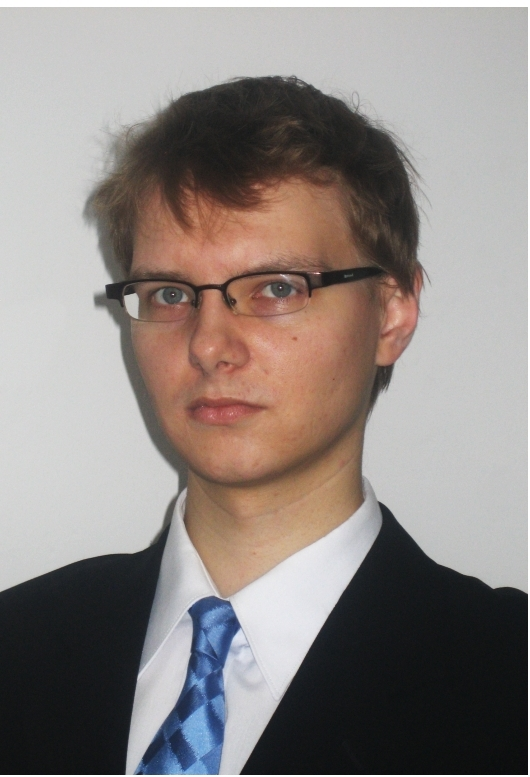
\includegraphics[height=6.5cm,width=4.5cm]{img/dyplom2.jpg} 
    \end{minipage}
    &
    \begin{minipage}{12cm}
    \begin{flushleft}
    \par\noindent\vspace{1\baselineskip} 
    \begin{tabular}[h]{l l}
    {\normalsize\it Specjalno��:} & Informatyka -- \\
    & In�ynieria oprogramowania \\
    & i~systemy informacyjne 
    \end{tabular}
    \par\noindent\vspace{1\baselineskip} 
    \begin{tabular}[h]{l l}
    {\normalsize\it Data urodzenia:} & {\normalsize 1 stycznia 1980~r.} 
    \end{tabular}
    \par\noindent\vspace{1\baselineskip}
    \begin{tabular}[h]{l l}
    {\normalsize\it Data rozpocz�cia studi�w:} & {\normalsize 1 pa�dziernika
    2004 r.}
    \end{tabular}
    \par\noindent\vspace{1\baselineskip}
    \end{flushleft}
    \end{minipage}
    \end{tabular}
    \vspace*{1\baselineskip}
    \begin{center}
	{\large\bfseries �yciorys}\par\bigskip
    \end{center}
    
    \indent
    Nazywam si�  \ldots.
    \par
    \vspace{2\baselineskip}
    \hfill\parbox{15em}{{\small\dotfill}\\[-.3ex]
    \centerline{\footnotesize podpis studenta}}\par
    \vspace{3\baselineskip}
    \begin{center}
 	{\large\bfseries Egzamin dyplomowy} \par\bigskip\bigskip
    \end{center}
    \par\noindent\vspace{1.5\baselineskip}
    Z�o�y� egzamin dyplomowy w dn. \dotfill 
    \par\noindent\vspace{1.5\baselineskip}
    Z wynikiem \dotfill 
    \par\noindent\vspace{1.5\baselineskip}
    Og�lny wynik studi�w \dotfill
    \par\noindent\vspace{1.5\baselineskip}
    Dodatkowe wnioski i uwagi Komisji \dotfill
    \par\noindent\vspace{1.5\baselineskip}
    \dotfill
    
    
     % �yciorys Wojtek
    \newpage\thispagestyle{empty}
    \begin{tabular}{p{5cm} p{12cm}}
    \begin{minipage}{5cm}
    \center
    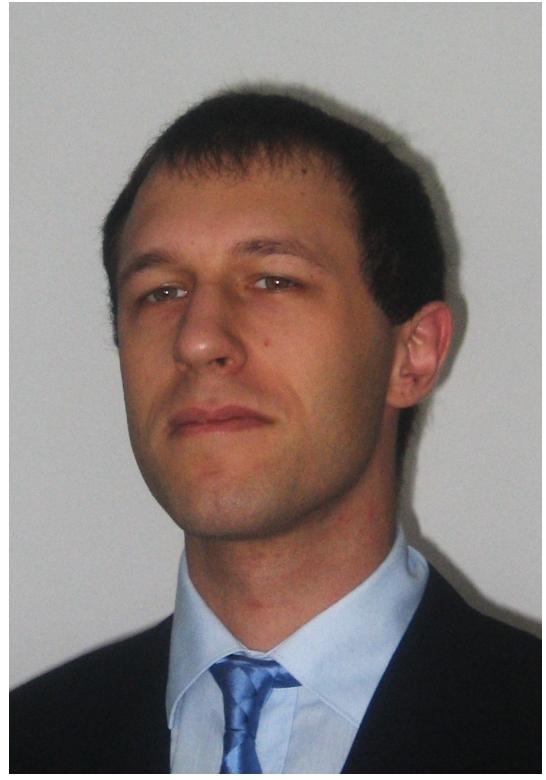
\includegraphics[height=6.5cm,width=4.5cm]{img/dyplom1.jpg} 
    \end{minipage}
    &
    \begin{minipage}{12cm}
    \begin{flushleft}
    \par\noindent\vspace{1\baselineskip} 
    \begin{tabular}[h]{l l}
    {\normalsize\it Specjalno��:} & Informatyka -- \\
    & In�ynieria oprogramowania \\
    & i~systemy informacyjne 
    \end{tabular}
    \par\noindent\vspace{1\baselineskip} 
    \begin{tabular}[h]{l l}
    {\normalsize\it Data urodzenia:} & {\normalsize 1 stycznia 1980~r.} 
    \end{tabular}
    \par\noindent\vspace{1\baselineskip}
    \begin{tabular}[h]{l l}
    {\normalsize\it Data rozpocz�cia studi�w:} & {\normalsize 1 pa�dziernika
    2004 r.}
    \end{tabular}
    \par\noindent\vspace{1\baselineskip}
    \end{flushleft}
    \end{minipage}
    \end{tabular}
    \vspace*{1\baselineskip}
    \begin{center}
	{\large\bfseries �yciorys}\par\bigskip
    \end{center}
    
    \indent
    Nazywam si�  \ldots.
    \par
    \vspace{2\baselineskip}
    \hfill\parbox{15em}{{\small\dotfill}\\[-.3ex]
    \centerline{\footnotesize podpis studenta}}\par
    \vspace{3\baselineskip}
    \begin{center}
 	{\large\bfseries Egzamin dyplomowy} \par\bigskip\bigskip
    \end{center}
    \par\noindent\vspace{1.5\baselineskip}
    Z�o�y� egzamin dyplomowy w dn. \dotfill 
    \par\noindent\vspace{1.5\baselineskip}
    Z wynikiem \dotfill 
    \par\noindent\vspace{1.5\baselineskip}
    Og�lny wynik studi�w \dotfill
    \par\noindent\vspace{1.5\baselineskip}
    Dodatkowe wnioski i uwagi Komisji \dotfill
    \par\noindent\vspace{1.5\baselineskip}
    \dotfill

    % Streszczenie
    \newpage\thispagestyle{empty}
    \vspace*{2\baselineskip}
    \begin{center}
	{\large\bfseries Streszczenie}\par\bigskip
    \end{center}
    
    {\itshape 
    Praca ta prezentuje \ldots}
    \vspace*{1\baselineskip}
    
    \noindent{\bf S�owa kluczowe}: {\itshape s�owa kluczowe.}
    \par
    \vspace{4\baselineskip}
    \begin{center}
	{\large\bfseries Abstract}\par\bigskip
    \end{center}
    \noindent{\bf Title}: {\itshape Thesis title.}\par
    \vspace*{1\baselineskip}
    {\itshape 
    This thesis describes \ldots}
    \vspace*{1\baselineskip}
       
    \noindent{\bf Key words}: {\itshape key words.}
   
\end{titlepage}

% ex: set tabstop=4 shiftwidth=4 softtabstop=4 noexpandtab fileformat=unix filetype=tex encoding=utf-8 fileencodings= fenc= spelllang=pl,en spell:

